\def\mcuWidth{10.5}
\def\mcuHeight{4}

\ctikzsubcircuitdef{spicMcu} {
    north, south, east, west,
    northeast, northwest, southeast, southwest,
    center,
    pin-01, pin-02, pin-03, pin-04, pin-05, pin-06, pin-07, pin-08, pin-09, pin-10,
    pin-11, pin-12, pin-13, pin-14, pin-15, pin-16, pin-17, pin-18, pin-19, pin-20,
    pin-21, pin-22, pin-23, pin-24, pin-25, pin-26, pin-27, pin-28, pin-29, pin-30,
    pin-31, pin-32, pin-33, pin-34, pin-35, pin-36, pin-37, pin-38, pin-39, pin-40%
} {
    coordinate (#1-origin)
    ++(5.25,-2)
    node [inner sep = 0pt, anchor = center] {
        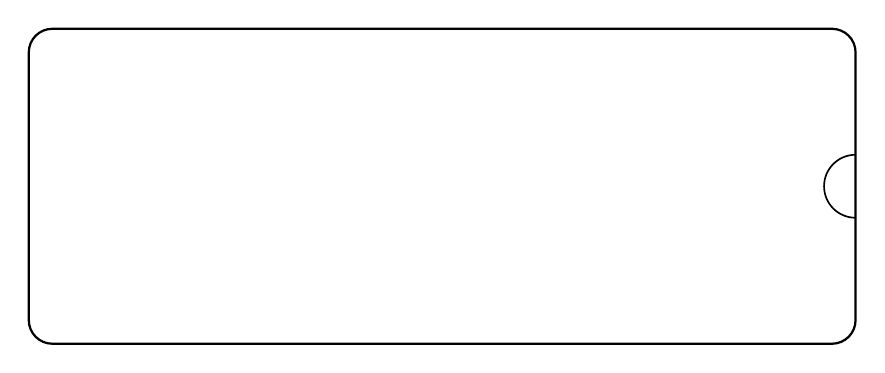
\begin{tikzpicture}
            \draw [rounded corners = 3mm, thick]
            (0,0) rectangle (\mcuWidth, -\mcuHeight)
            (0,0) coordinate (origin)
            ;
            %% \foreach \x in {0.5,1.0,...,10} {
            %%     \draw (origin) ++(\x, 0) -- ++(0,0.25);
            %%     \draw (origin) ++(\x, -4) -- ++(0,-0.25);
            %% }
            \draw [semithick]
            (origin) ++(\mcuWidth,-2)
            ++(0,0.4)
            arc [start angle = 90, end angle = 270, radius = 0.4]
            ;
        \end{tikzpicture}
    }
    (#1-origin) ++(0.5,0.25) coordinate (#1-pin-20)
    (#1-origin) ++(1.0,0.25) coordinate (#1-pin-19)
    (#1-origin) ++(1.5,0.25) coordinate (#1-pin-18)
    (#1-origin) ++(2.0,0.25) coordinate (#1-pin-17)
    (#1-origin) ++(2.5,0.25) coordinate (#1-pin-16)
    (#1-origin) ++(3.0,0.25) coordinate (#1-pin-15)
    (#1-origin) ++(3.5,0.25) coordinate (#1-pin-14)
    (#1-origin) ++(4.0,0.25) coordinate (#1-pin-13)
    (#1-origin) ++(4.5,0.25) coordinate (#1-pin-12)
    (#1-origin) ++(5.0,0.25) coordinate (#1-pin-11)
    (#1-origin) ++(5.5,0.25) coordinate (#1-pin-10)
    (#1-origin) ++(6.0,0.25) coordinate (#1-pin-09)
    (#1-origin) ++(6.5,0.25) coordinate (#1-pin-08)
    (#1-origin) ++(7.0,0.25) coordinate (#1-pin-07)
    (#1-origin) ++(7.5,0.25) coordinate (#1-pin-06)
    (#1-origin) ++(8.0,0.25) coordinate (#1-pin-05)
    (#1-origin) ++(8.5,0.25) coordinate (#1-pin-04)
    (#1-origin) ++(9.0,0.25) coordinate (#1-pin-03)
    (#1-origin) ++(9.5,0.25) coordinate (#1-pin-02)
    (#1-origin) ++(10.0,0.25) coordinate (#1-pin-01)
    %% Bottom pins
    (#1-origin) ++(0.5,-\mcuHeight) ++(0,-0.25) coordinate (#1-pin-21)
    (#1-origin) ++(1.0,-\mcuHeight) ++(0,-0.25) coordinate (#1-pin-22)
    (#1-origin) ++(1.5,-\mcuHeight) ++(0,-0.25) coordinate (#1-pin-23)
    (#1-origin) ++(2.0,-\mcuHeight) ++(0,-0.25) coordinate (#1-pin-24)
    (#1-origin) ++(2.5,-\mcuHeight) ++(0,-0.25) coordinate (#1-pin-25)
    (#1-origin) ++(3.0,-\mcuHeight) ++(0,-0.25) coordinate (#1-pin-26)
    (#1-origin) ++(3.5,-\mcuHeight) ++(0,-0.25) coordinate (#1-pin-27)
    (#1-origin) ++(4.0,-\mcuHeight) ++(0,-0.25) coordinate (#1-pin-28)
    (#1-origin) ++(4.5,-\mcuHeight) ++(0,-0.25) coordinate (#1-pin-29)
    (#1-origin) ++(5.0,-\mcuHeight) ++(0,-0.25) coordinate (#1-pin-30)
    (#1-origin) ++(5.5,-\mcuHeight) ++(0,-0.25) coordinate (#1-pin-31)
    (#1-origin) ++(6.0,-\mcuHeight) ++(0,-0.25) coordinate (#1-pin-32)
    (#1-origin) ++(6.5,-\mcuHeight) ++(0,-0.25) coordinate (#1-pin-33)
    (#1-origin) ++(7.0,-\mcuHeight) ++(0,-0.25) coordinate (#1-pin-34)
    (#1-origin) ++(7.5,-\mcuHeight) ++(0,-0.25) coordinate (#1-pin-35)
    (#1-origin) ++(8.0,-\mcuHeight) ++(0,-0.25) coordinate (#1-pin-36)
    (#1-origin) ++(8.5,-\mcuHeight) ++(0,-0.25) coordinate (#1-pin-37)
    (#1-origin) ++(9.0,-\mcuHeight) ++(0,-0.25) coordinate (#1-pin-38)
    (#1-origin) ++(9.5,-\mcuHeight) ++(0,-0.25) coordinate (#1-pin-39)
    (#1-origin) ++(10.0,-\mcuHeight) ++(0,-0.25) coordinate (#1-pin-40)
    %% geo coordinates
    \markgeocoordinate {#1}
    {(#1-pin-01)} {(#1-pin-30)}
    {(#1-origin)} {(#1-origin) ++(\mcuWidth,-\mcuHeight)}
}

\newcommand\ovrMcuPinHoles[1] {
    (#1-pin-01) node [ocirc] {}
    (#1-pin-02) node [ocirc] {}
    (#1-pin-03) node [ocirc] {}
    (#1-pin-04) node [ocirc] {}
    (#1-pin-05) node [ocirc] {}
    (#1-pin-06) node [ocirc] {}
    (#1-pin-07) node [ocirc] {}
    (#1-pin-08) node [ocirc] {}
    (#1-pin-09) node [ocirc] {}
    (#1-pin-10) node [ocirc] {}
    (#1-pin-11) node [ocirc] {}
    (#1-pin-12) node [ocirc] {}
    (#1-pin-13) node [ocirc] {}
    (#1-pin-14) node [ocirc] {}
    (#1-pin-15) node [ocirc] {}
    (#1-pin-16) node [ocirc] {}
    (#1-pin-17) node [ocirc] {}
    (#1-pin-18) node [ocirc] {}
    (#1-pin-19) node [ocirc] {}
    (#1-pin-20) node [ocirc] {}
    (#1-pin-21) node [ocirc] {}
    (#1-pin-22) node [ocirc] {}
    (#1-pin-23) node [ocirc] {}
    (#1-pin-24) node [ocirc] {}
    (#1-pin-25) node [ocirc] {}
    (#1-pin-26) node [ocirc] {}
    (#1-pin-27) node [ocirc] {}
    (#1-pin-28) node [ocirc] {}
    (#1-pin-29) node [ocirc] {}
    (#1-pin-30) node [ocirc] {}
    (#1-pin-31) node [ocirc] {}
    (#1-pin-32) node [ocirc] {}
    (#1-pin-33) node [ocirc] {}
    (#1-pin-34) node [ocirc] {}
    (#1-pin-35) node [ocirc] {}
    (#1-pin-36) node [ocirc] {}
    (#1-pin-37) node [ocirc] {}
    (#1-pin-38) node [ocirc] {}
    (#1-pin-39) node [ocirc] {}
    (#1-pin-40) node [ocirc] {}
}

\ctikzsubcircuitactivate{spicMcu}
